\documentclass[10pt]{article}

\usepackage{amsmath}

\newcommand{\myvec}[1]{\ensuremath{\begin{pmatrix}#1\end{pmatrix}}}

\newcommand{\mydet}[1]{\ensuremath{\begin{vmatrix}#1\end{vmatrix}}}

\newcommand{\solution}{\noindent \textbf{Solution: }}

\providecommand{\brak}[1]{\ensuremath{\left(#1\right)}}

\providecommand{\norm}[1]{\left\lVert#1\right\rVert}
\usepackage{graphicx}
\usepackage{float}

\let\vec\mathbf

\title{Coordinate Geometry}
\author{G.sai avinash (gsavinash@sriprakashschools.com)}

\begin{document}
\maketitle
\section*{Class 10$^{th}$ Maths - Chapter 7}
This is Problem-7 from Exercise 7.4
\begin{enumerate}
\item   Let A(4, 2), B(6,5) and C(1, 4) be the vertices of triangle ABC\\
(ii)Find the coordinates of the point P on the AD, such that \\
AP: PD = 2: 1.\\
\solution Median AD of the triangle will divide the side BC in two equal parts. So D is the midpoint of side BC\\ 
\begin{align}
\vec{D} &= \frac{(m)\vec{B} + (n)\vec{C}}{m+n}\\
\vec{D} &= \frac{1\myvec{6\\5} + 1\myvec{1\\4}}{2}\\
\vec{D} &= \myvec{\frac{7}{2}\\\frac{9}{2}}\\
\end{align}

Point P divides the side AD in a ratio 2:1\\
\begin{align}
\vec{P} &=\frac{(m)\vec{D}+(n)\vec{A}}{m+n}\\
\vec{P} &=\frac{(2)\myvec{\frac{7}{2}\\\frac{9}{2}}+(1)\myvec{4\\2}}{3}\\
\vec{P} &=\myvec{\frac{11}{3}\\\frac{11}{3}}\\
\end{align}
\end{enumerate}
\begin{figure}[H]
			\centering
			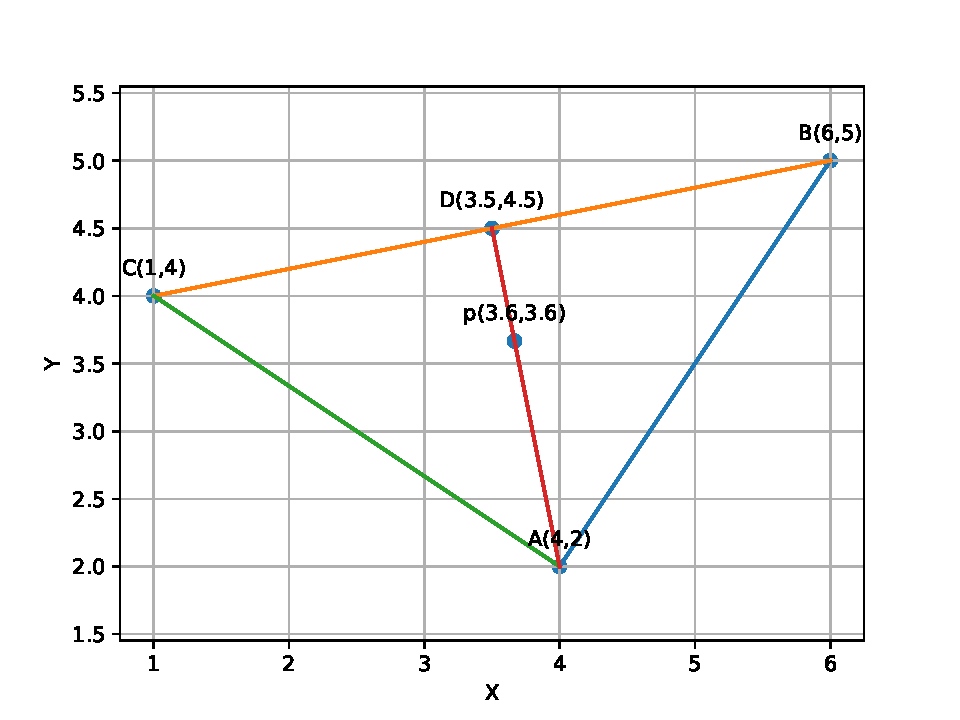
\includegraphics[width=\columnwidth]{figs/fig.pdf}
			\caption{Triangle ABC}
			\label{fig:9}
		\end{figure}
\end{document}
